\section{\numb section 7. Finite elements and integrators}


Finite elments are still incipient in \maniFEM.
Paragraph \numb section 7.\numb parag 1 discusses the concept of finite element
and paragraph \numb section 7.\numb parag 2 gives an example of rudimentary use.
There is a lot of ongoing work on this subject.


\paragraph{\numb section 7.\numb parag 1. Finite elements}

The notion of a finite element is quite complex.
The purpose of a {\codett FiniteElement} is to build a list of functions, say, $ \psi $,
defined on our mesh.
The linear span of these functions will be a discretized Hilbert space.
It is the {\codett FiniteElement}'s job to replace, in the variational formulation,
the unknown function by one $ \psi $, the test function by another $ \psi $ and,
by evaluating the integrals, obtain the coefficients of a system of linear equations.
Some external solver will then solve the system, and it is the job of the finite element
to transform back the vector produced by the solver into a function defined on our mesh.

Computing each integral is a somewhat separate process; it's the job of an {\codett Integrator}
which could be a Gauss quadrature or some other procedure like symbolic integration.
When a Gauss quadrature is used, the separation between a {\codett FiniteElement}'s job
and the {\codett Itegrator}'s job is not very sharp because often the Gauss quadrature is
perfomed not on the physical cell but rather on a master element which is built and
handled by the {\codett FiniteElement}.
The authors of {\maniFEM} have tried to separate these two concepts
as much as possible, especially because some users may want to use a {\codett FiniteElement}
with no master element, or an {\codett Integrator} acting directly on the physical cell.

Thus, there is a base class {\codett FiniteElement} and a derived class
{\codett FiniteElement::withMaster} which keeps, as an extra attribute, the map transforming
the master element to the current physical cell.
This map depends of course on the geometry of the cell and thus it must be computed from
scratch each time we begin integrating on a new cell.
We say that the {\codett FiniteElement} is docked on a new {\codett Cell};
the method {\codett dock\_on} performs this operation.
This method is element-specific, each type of finite element having its own class.

For instance, the class {\codett FiniteElement::Lagrange\_Q1} is a class derived from
\hfil\break{\codett FiniteElement::withMaster}.
It will only {\codett dock\_on} quadrilaterals (two-dimensional {\codett Cell}s
with four sides).
% Recall that in {\maniFEM} the vertices do not have necessarily any number attached.
% When we create a {\codett FiniteElement::Lagrange\_Q1} object, it will enumerate vertices
% of the mesh if a mesh exists already, and it will prepare the ground for vertices created
% in the future to be enumerated, too.
% This enumeration is useful to identify a vector of real numbers with the values
% (at each vertex) of a function defined on the mesh.
When docking on a cell, the {\codett FiniteElement::Lagrange\_Q1} object will build four
``shape functions'' and a transformation map (a diffeomorphism between a master element
occuppying the square $ [-1, 1]^2 $ and the current cell).
It will also build the jacobian of this transformation map.
The four shape functions can be accessed through the method {\codett basis\_function},
as shown in paragraph \numb section 7.\numb parag 2.


\paragraph{\numb section 7.\numb parag 2. A rudimentary example}

Let's look at an example about the Laplace operator with non-homogeneous Dirichlet
boundary conditions.

It should be stressed that the approach presented in this paragraph is rather low-level.
We are working hard to make {\maniFEM} understand statements describing variational
formulations given as {\tt C++} objects.
When this part of the code is done, the programming style will become much more elegant
and compact.

\vfil\eject
\verbatim
   Manifold RR2 ( tag::Euclid, tag::of_dim, 2 );
   Function xy = RR2.build_coordinate_system ( tag::Lagrange, tag::of_degree, 1 );
   Function x = xy[0],  y = xy[1];

   // build a 10x12 mesh on a square domain
   Cell A ( tag::vertex );  x(A) = 0.;   y(A) = 0.;
   Cell B ( tag::vertex );  x(B) = 1.;   y(B) = 0.;
   Cell C ( tag::vertex );  x(C) = 1.;   y(C) = 1.;
   Cell D ( tag::vertex );  x(D) = 0.;   y(D) = 1.;
   Mesh AB ( tag::segment, A.reverse(), B, tag::divided_in, 10 );
   Mesh BC ( tag::segment, B.reverse(), C, tag::divided_in, 12 );
   Mesh CD ( tag::segment, C.reverse(), D, tag::divided_in, 10 );
   Mesh DA ( tag::segment, D.reverse(), A, tag::divided_in, 12 );
   Mesh ABCD ( tag::rectangle, AB, BC, CD, DA );

   // declare the type of finite element
   FiniteElement fe
      ( tag::with_master, tag::quadrangle, tag::Lagrange, tag::of_degree, 1 );
   Integrator integ = fe.set_integrator ( tag::Gauss, tag::quad_4 );
\endverbatim

Vertices are not numbered. In the future, a more elegant solution for automatic numbering
of vertices will be implemented; for now, we build a map {\codett numbering} (see the source
code in file {\codett main-\numb section 7.\numb parag 2.cpp} in the distribution tree),
to be used as shown below.
The matrix of the linear system and the vector holding the free coefficients
are declared as objects of the {\codett Eigen} library.

\verbatim
   size_t size_matrix = ABCD.number_of ( tag::vertices );
   assert ( size_matrix == numbering.size() );
   Eigen::SparseMatrix <double> matrix_A ( size_matrix, size_matrix );
   Eigen::VectorXd vector_b ( size_matrix );  vector_b.setZero();
\endverbatim

We now run over all rectangular cells of {\codett ABCD}, dock the finite element,
compute integrals of the form $ \displaystyle \int\!\!\!\int {\partial \psi_i \over
\partial x_\alpha} {\partial \psi_j \over \partial x_\beta} dx $ and add the obtained
values to the global matrix:

\verbatim
   // run over all square cells composing ABCD
   CellIterator it = ABCD.iter_over ( tag::cells_of_dim, 2 );
   for ( it.reset(); it.in_range(); it++ )
   {  Cell small_square = *it;
      fe.dock_on ( small_square );
      // run twice over the four vertices of 'small_square'
      CellIterator it1 = small_square.boundary().iter_over ( tag::vertices );
      CellIterator it2 = small_square.boundary().iter_over ( tag::vertices );
      for ( it1.reset(); it1.in_range(); it1++ )
      for ( it2.reset(); it2.in_range(); it2++ )
      {  Cell V = *it1, W = *it2;
         // V may be the same as W, no problem about that
         Function psiV = fe.basis_function(V),
                  psiW = fe.basis_function(W),
                  d_psiV_dx = psiV.deriv(x),
                  d_psiV_dy = psiV.deriv(y),
                  d_psiW_dx = psiW.deriv(x),
                  d_psiW_dy = psiW.deriv(y);
\endverbatim

\vfil\eject
\verbatim
         // 'fe' is already docked on 'small_square'
         // so this will be the domain of integration
         matrix_A.coeffRef ( numbering[V.core]-1, numbering[W.core]-1 ) +=
            fe.integrate ( d_psiV_dx * d_psiW_dx + d_psiV_dy * d_psiW_dy );      }  }
\endverbatim

In the above, {\codett coeffRef} is the method used by {\codett Eigen} to access elements of
a sparse matrix.

We impose Dirichlet boundary conditions $ u(x,y) = xy $ (this way, we know beforehand
the exact solution will be $ u(x,y) = xy $).
We use a function {\codett impose\_value\_of\_unknown} which changes the {\codett matrix\_A}
and the {\codett vector\_b} in order to impose the Dirichlet condition {\codett u(i) = 
some\_value}. See the source code in file {\codett main-\numb section 7.\numb parag 2.cpp}
in the distribution tree for the definition of the {\codett impose\_value\_of\_unknown}
function.

\verbatim
   CellIterator it = BC.iter_over ( tag::vertices );
   for ( it.reset(); it.in_range(); it++ )
   {   Cell P = *it;
       size_t i = numbering[P.core]-1;
       impose_value_of_unknown ( matrix_A, vector_b, i, y(P) );  }
\endverbatim

We then use {\codett Eigen} to solve the system of linear equations :

\verbatim
   Eigen::ConjugateGradient < Eigen::SparseMatrix<double>,
                              Eigen::Lower|Eigen::Upper    > cg;
   cg.compute ( matrix_A );
   Eigen::VectorXd u = cg.solve ( vector_b );
\endverbatim

And obtain the expected solution :

\bigskip
{ \psfrag{A}{\special{ps: gsave 0 0 0.8 setrgbcolor}{\codett A}\special{ps: grestore}}
\psfrag{B}{\special{ps: gsave 0 0 0.8 setrgbcolor}{\codett B}\special{ps: grestore}}
\psfrag{C}{\special{ps: gsave 0 0 0.8 setrgbcolor}{\codett C}\special{ps: grestore}}
\psfrag{D}{\special{ps: gsave 0 0 0.8 setrgbcolor}{\codett D}\special{ps: grestore}}
\centerline{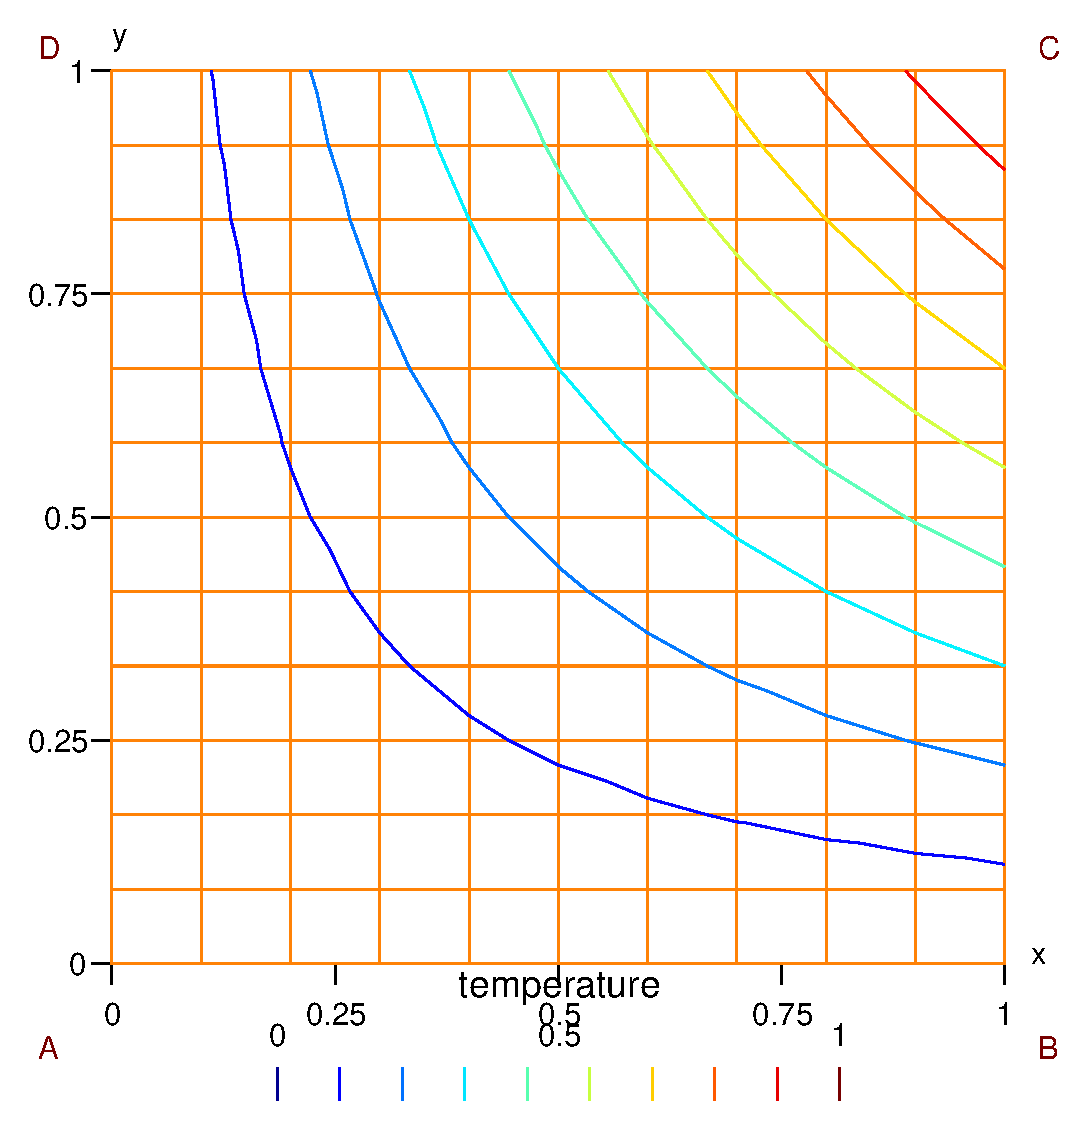
\includegraphics[width=60mm]{square-Dirichlet.eps}} }

We stress again that this example shows a rather rudimentary way of using finite elements in
\maniFEM.
We are working hard to reach a more elegant, compact and high-level style.
For instance, the numbering of vertices should be automated.
Also, the user should have the possibility to declare the partial differential equation
through a compact declaration of the corresponding variational formulation.

Another limitation of {\maniFEM} is that, at present, finite element computations
are rather slow.
This is so because each docking operation implies a lot of symbolic calculations;
the same happens when we differentiate and then integrate functions.
There are two ways of circunventing this limitation.
The first one is : if your mesh is made of identical finite elements
(like the example in the present paragraph), you can compute the elementary matrix
just once and then assembly the global matrix from it.
It will surely be much faster.
A second way around is a deep optimization of the {\maniFEM} library,
object of on-going work.
A significant part of the symbolic calculations should be done just once,
when the finite element is declared.
Only a small chunk of symbolic computation will be performed at docking and
later, when we build the elementary matrix.

